\documentclass{article}
\usepackage[mast]{dennis}

\title{Solutions to Lengths and Areas in Triangles}
\author{Dennis Chen}
\date{GQU}

\begin{document}
\maketitle

\toc

\pagebreak\section{Unsourced}
Find the inradius of the triangles with the following lengths:
    
    \begin{itemize}
        \Item $3,4,5$
        
        \Item $5,12,13$
        
        \Item $13,14,15$
        
        \Item $5,7,8$
    \end{itemize}

    (These are arranged by difficulty. All of these are good to know.)
    
\subsection{Solution}
We find the area of each of the triangles and divide by the semiperimeter.
\begin{itemize}
\Item This is a right triangle, so the area is $\frac{3\cdot 4}{2}=6.$ Thus the inradius is $\frac{6}{\frac{3+4+5}{2}}=1.$

\Item This is a right triangle, so the area is $\frac{5\cdot 12}{2}=30.$ Thus the inradius is $\frac{30}{\frac{5+12+13}{2}}=2.$

\Item By Heron's Formula, the area of this triangle is $\sqrt{21(21-13)(21-14)(21-15)}=84.$ Thus the inradius is $\frac{84}{\frac{13+14+15}{2}}=4.$

\Item By Heron's Formula, the area of this triangle is $\sqrt{10(10-5)(10-7)(10-8)}=10\sqrt{3}.$ Thus the inradius is $\frac{10\sqrt{3}}{\frac{5+7+8}{2}}=\sqrt{3}.$
\end{itemize}

\pagebreak\section{Unsourced}
Prove that in a right triangles with legs of length $a,b,$ and hypotenuse with length $c,$ $r=\frac{a+b-c}{2}.$

\subsection{Solution}
Let the triangle have legs $AC,BC$ and hypotenuse $AB,$ let the incenter of $\triangle ABC$ be $I,$ and let the incircle be tangent to $AC,BC$ at $X,Y.$ Then note that $CXOY$ is a square, since $\angle XCY=90^{\circ}$ and $\angle OXC=\angle OYC=90^{\circ}$ because $AC,BC$ are tangents. So $r=s-c=\frac{a+b-c}{2}.$

\begin{center}
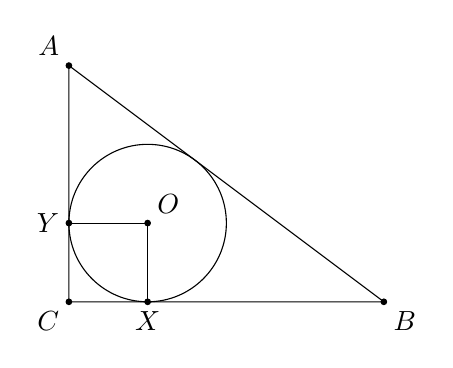
\begin{tikzpicture}
\draw (0,0)--(4,0)--(0,3)--cycle;
\filldraw (0,0) circle (1pt) node[anchor=north east] {$C$};
\filldraw (4,0) circle (1pt) node[anchor=north west] {$B$};
\filldraw (0,3) circle (1pt) node[anchor=south east] {$A$};
\draw (1,1) circle (1);

\filldraw (1,0) circle (1pt) node[anchor=north] {$X$};
\filldraw (0,1) circle (1pt) node[anchor=east] {$Y$};
\filldraw (1,1) circle (1pt) node[anchor=south west] {$O$};
\draw (1,0)--(1,1)--(0,1);
\end{tikzpicture}
\end{center}

\pagebreak\section{Unsourced}
In $\triangle ABC,$ $AB=5,$ $BC=12,$ and $CA=13.$ Points $D,E$ are on $BC$ such that $BD=DC$ and $\angle BAE=\angle CAE.$ Find $[ADE].$

\subsection{Solution}

Note that by the angle bisector theorem, $BE=\frac{5}{5+13}\cdot 12=\frac{10}{3},$ so $ED=\frac{8}{3}.$ Thus $[ADE]=\frac{1}{2}\cdot\frac{8}{3}\cdot 5=\frac{20}{3}.$

\begin{center}
\begin{tikzpicture}[scale=0.3]
\filldraw[color=thmblue] (10/3,0)--(6,0)--(0,5)--cycle;

\draw (0,0)--(12,0)--(0,5)--cycle;
\filldraw (0,0) circle (3pt) node[anchor=north east]{$B$};
\filldraw (12,0) circle (3pt) node[anchor=north west]{$C$};
\filldraw (0,5) circle (3pt) node[anchor=south east]{$A$};
\filldraw (6,0) circle (3pt) node[anchor=north]{$D$};
\filldraw (10/3,0) circle (3pt) node[anchor=north]{$E$};
\draw(10/3,0)--(0,5)--(6,0);
\end{tikzpicture}
\end{center}

\pagebreak\section{Unsourced}
Find the maximum area of a triangle with two of its sides having lengths $10,11.$

\subsection{Solution}
By $\frac{1}{2}ab\sin C,$ the area is $\frac{1}{2}\cdot 10\cdot 11\cdot \sin\theta=55\sin\theta,$ where $\theta$ is the angle between the sides of lengths $10,11.$ Clearly $\sin\theta$ is maximized when $\theta=90^{\circ},$ so the maximum area is $55.$

\pagebreak\section{e-dchen Mock MATHCOUNTS, Sprint Round, Problem 17}
Consider rectangle $ABCD$ such that $AB=2$ and $BC=1.$ Let $X,Y$ trisect $AB.$ Then let $DX$ and $DY$ intersect $AC$ at $P$ and $Q,$ respectively. What is the area of quadrilateral $XYQP?$

\subsection{Solution}
Without loss of generality, let $AX<AY.$ Then note that we want to find $[AQY]-[APX].$ Since $\triangle AQY\sim \triangle CQD,$ the height from $Q$ to $AY$ is $\frac{2}{5}$ and since $\triangle APX\sim \triangle CPD,$ the height from $P$ to $AX$ is $\frac{1}{4}.$ Thus $[AQY]=\frac{1}{2}\cdot\frac{4}{3}\cdot\frac{2}{5}=\frac{4}{15}$ and $[APX]=\frac{1}{2}\cdot\frac{2}{3}\cdot\frac{1}{4}=\frac{1}{12},$ so $[PQXY]=\frac{4}{15}-\frac{1}{12}=\frac{11}{60}.$

\begin{center}
\begin{tikzpicture}[scale=1.5]
\filldraw[color=thmblue] (4/5,2/5)--(1/2,1/4)--(2/3,0)--(4/3,0)--cycle;

\draw (0,0)--(2,0)--(2,1)--(0,1)--cycle;
\draw (0,0)--(2,1);
\draw (2/3,0)--(0,1)--(4/3,0);
\filldraw (0,0) circle (1pt) node[anchor=north east]{$A$};
\filldraw (2,0) circle (1pt) node[anchor=north west]{$B$};
\filldraw (2,1) circle (1pt) node[anchor=south west]{$C$};
\filldraw (0,1) circle (1pt) node[anchor=south east]{$D$};
\filldraw (2/3,0) circle (1pt) node[anchor=north]{$X$};
\filldraw (4/3,0) circle (1pt) node[anchor=north]{$Y$};
\filldraw (1/2,1/4) circle (1pt) node[anchor=east]{$P$};
\filldraw (4/5,2/5) circle (1pt) node[anchor=south]{$Q$};
\end{tikzpicture}
\end{center}

\pagebreak\section{Autumn Mock AMC 10, Problem 8}
Equilateral triangle $ABC$ has side length $6$. Points $D, E, F$ lie within the lines $AB, BC$ and $AC$ such that $BD=2AD$, $BE=2CE$, and $AF=2CF$. Let $N$ be the numerical value of the area of triangle $DEF$. Find $N^2$.

\subsection{Solution}

We know that $[ABC]=9\sqrt{3}.$ By $\frac{1}{2}ab\sin\theta,$
\[[AFD]=\frac{1}{2}\cdot 4\cdot 2\sin 60^{\circ}=2\sqrt{3}\]
\[[BDE]=\frac{1}{2}\cdot 4\cdot 4\sin 60^{\circ}=4\sqrt{3}\]
\[[CEF]=\frac{1}{2}\cdot 2\cdot 2\sin 60^{\circ}=\sqrt{3}.\]
Thus $[ABC]=9\sqrt{3}-2\sqrt{3}-4\sqrt{3}-\sqrt{3}=2\sqrt{3},$ so the answer is $12.$

\begin{center}
\begin{tikzpicture}[scale=0.6]
\filldraw[color=thmblue] (4,0)--(5,1.73205081)--(2,3.46410162)--cycle;
\draw (0,0)--(6,0)--(3,5.19615242)--cycle;
\draw (4,0)--(5,1.73205081)--(2,3.46410162)--cycle;

\filldraw (0,0) circle (2pt) node[anchor=north east]{$B$};
\filldraw (6,0) circle (2pt) node[anchor=north west]{$C$};
\filldraw (3,5.19615242) circle (2pt) node[anchor=south]{$A$};

\filldraw (5,1.73205081) circle (2pt) node[anchor=west]{$F$};
\filldraw (4,0) circle (2pt) node[anchor=north]{$E$};
\filldraw (2,3.46410162) circle (2pt) node[anchor=east]{$D$};
\end{tikzpicture}
\end{center}

\pagebreak\section{AIME I 2019/3}
In $\triangle PQR$, $PR=15$, $QR=20$, and $PQ=25$. Points $A$ and $B$ lie on $\overline{PQ}$, points $C$ and $D$ lie on $\overline{QR}$, and points $E$ and $F$ lie on $\overline{PR}$, with $PA=QB=QC=RD=RE=PF=5$. Find the area of hexagon $ABCDEF$.

\subsection{Solution}
We know that $[PQR]=150.$ By $\frac{1}{2}ab\sin\theta,$
\[[PFA]=\frac{1}{2}\cdot 5\cdot 5\sin \angle APF=\frac{1}{2}\cdot 5\cdot 5\cdot\frac{4}{5}=10\]
\[[QBC]=\frac{1}{2}\cdot 5\cdot 5\sin \angle BQC=\frac{1}{2}\cdot 5\cdot 5\cdot \frac{3}{5}=\frac{15}{2}\]
\[[RDE]=\frac{1}{2}\cdot 5\cdot 5\sin \angle DRE=\frac{1}{2}\cdot 5\cdot 5\cdot 1=\frac{25}{2}.\]
Thus $[ABC]=150-10-\frac{15}{2}-\frac{25}{2}=120.$

\begin{center}
\begin{tikzpicture}[scale=0.2]
\filldraw[color=thmblue] (0,5)--(5,0)--(15,0)--(16,3)--(4,12)--(0,10)--cycle;
\draw (0,0)--(20,0)--(0,15)--cycle;
\draw (0,5)--(5,0)--(15,0)--(16,3)--(4,12)--(0,10)--cycle;

\filldraw (0,0) circle (5pt) node[anchor=north east]{$R$};
\filldraw (0,15) circle (5pt) node[anchor=south east]{$P$};
\filldraw (20,0) circle (5pt) node[anchor=north west]{$Q$};

\filldraw (4,12) circle (5pt) node[anchor=south west]{$A$};
\filldraw (16,3) circle (5pt) node[anchor=south west]{$B$};
\filldraw (15,0) circle (5pt) node[anchor=north]{$C$};
\filldraw (5,0) circle (5pt) node[anchor=north]{$D$};
\filldraw (0,5) circle (5pt) node[anchor=east]{$E$};
\filldraw (0,10) circle (5pt) node[anchor=east]{$F$};
\end{tikzpicture}
\end{center}

\pagebreak\section{AMC 8 2019/24}
In triangle $ABC$, point $D$ divides side $\overline{AC}$ so that $AD:DC=1:2$. Let $E$ be the midpoint of $\overline{BD}$ and let $F$ be the point of intersection of line $BC$ and line $AE$. Given that the area of $\triangle ABC$ is $360$, what is the area of $\triangle EBF$?
\begin{center}
\begin{asy}
import olympiad;
size(5cm);
pair A,B,C,DD,EE,FF;
B = (0,0); C = (3,0); 
A = (1.2,1.7);
DD = (2/3)*A+(1/3)*C;
EE = (B+DD)/2;
FF = intersectionpoint(B--C,A--A+2*(EE-A));
draw(A--B--C--cycle);
draw(A--FF); 
draw(B--DD);dot(A); 
label("$A$",A,N);
dot(B); 
label("$B$",
B,SW);dot(C); 
label("$C$",C,SE);
dot(DD); 
label("$D$",DD,NE);
dot(EE); 
label("$E$",EE,NW);
dot(FF); 
label("$F$",FF,S);
\end{asy}
\end{center}

\subsection{Solution}
We use mass points. Note that we can assign $\diamond A=\diamond C=1,$ implying $\diamond D=2,$ which leads to $\diamond B=2$ and $\diamond E=4.$ Thus $\diamond F=3.$

Now note that $[EBF]=[ABC]\cdot\frac{EF}{AF}\cdot\frac{BF}{BC}$ by $\frac{bh}{2},$ and that
\[[ABC]\cdot\frac{EF}{AF}\cdot\frac{BF}{BC}=360\cdot\frac{1}{4}\cdot\frac{1}{3}=30\]
by mass points.

\pagebreak\section{Unsourced}
Consider $\triangle ABC$ such that $AB=8,$ $BC=5,$ and $CA=7.$ Let $AB$ and $CA$ be tangent to the incircle at $T_C,$ $T_B,$ respectively. Find $[AT_BT_C].$

\subsection{Solution}
The gist of the solution is that we use Heron's to find that $[ABC]=10\sqrt{3},$ use the Two Tangent Theorem to find $AT_B=AT_C=5,$ and use $\frac{1}{2}ab\sin \theta$ to find $\frac{[AT_BT_C]}{[ABC]},$ which determines $[AT_BT_C].$

We first prove the following lemma, which we have implicitly used on the problems before this.

\begin{lemma}[Area Ratio Given Collinear Points]
Given collinear points $P,A,X$ and $P,B,Y,$
\[\frac{[PXY]}{[PAB]}=\frac{PX\cdot PY}{PA\cdot PB}.\]
\end{lemma}

\begin{pro}
Note that $[PXY]=\frac{1}{2}PX\cdot PY\sin\angle XPY$ and $[PAB]=\frac{1}{2}PA\cdot PB\sin\angle APB,$ and since $P,A,X$ and $P,B,Y$ are collinear, $\sin\angle XPY=\sin\angle APB,$ which proves our desired result.
\end{pro}

Now note that $\frac{[AT_BT_C]}{[ABC]}=\frac{5\cdot 5}{7\cdot 8},$ implying that $[AT_BT_C]=\frac{125\sqrt{3}}{28}.$

\begin{center}
\begin{tikzpicture}[scale=0.6]
\filldraw[color=thmblue] (4.7143,1.9795)--(1.5,2.5981)--(4,{4*sqrt(3)})--cycle;

\draw (0,0)--(5,0)--(4,{4*sqrt(3)})--cycle;
\draw (3,{sqrt(3)}) circle ({sqrt(3)});
\draw[dotted] (4.7143,1.9795)--(1.5,2.5981);

\filldraw (0,0) circle (2pt) node[anchor=north east]{$B$};
\filldraw (5,0) circle (2pt) node[anchor=north west]{$C$};
\filldraw (4,{4*sqrt(3)}) circle (2pt) node[anchor=south]{$A$};

\filldraw (4.7143,1.9795) circle (2pt) node[anchor=south west]{$T_B$};
\filldraw (1.5,2.5981) circle (2pt) node[anchor=south east]{$T_C$};
\end{tikzpicture}
\end{center}

\pagebreak\section{Unsourced}
Consider trapezoid $ABCD$ with bases $AB$ and $CD.$ If $AC$ and $BD$ intersect at $P,$ prove the sum of the areas of $\triangle ABP$ and $\triangle CDP$ is at least half the area of trapezoid $ABCD.$

\subsection{Solution}

Let $AB=b_1,$ $CD=b_2,$ and let the height from $P$ to $AB$ be $h_1$ and the height from $P$ to $CD$ be $h_2.$ Note that we want to prove
\[\frac{b_1h_1+b_2h_2}{2}\geq \frac{(b_1+b_2)(h_1+h_2)}{4},\]
which is equivalent to
\[2b_1h_1+2b_2h_2\geq b_1h_1+b_2h_2+b_1h_2+b_2h_1\]
\[b_1h_1+b_2h_2\geq b_1h_2+b_2h_1.\]
Note that by similar triangles, $b_2=b_1k$ and $h_2=h_1k$ for some constant $k.$ So this is equivalent to
\[b_1h_1(1+k^2)\geq b_1h_1(2k)\]
\[k^2+1\geq 2k\]
\[(k-1)^2\geq 0,\]
and the last inequality is obviously true. Since all steps are reversible, we are done.

\begin{center}
\begin{tikzpicture}[scale=1.4]
\filldraw[color=thmblue] (0.5,1.5)--(1.5,1.5)--(1,1)--cycle;
\filldraw[color=thmblue] (0,0)--(1,1)--(2,0)--cycle;

\draw (0,0)--(0.5,1.5)--(1.5,1.5)--(2,0)--cycle;
\draw[color=darkmidnightblue] (0,0)--(1.5,1.5);
\draw[color=darkmidnightblue] (2,0)--(0.5,1.5);

\draw[color=sangria,dotted] (1,1.5)--(1,0);

\node at (1,0) [anchor=north] {$b_2$};
\node at (1,1.5) [anchor=south] {$b_1$};

\node at (1,0.35) [anchor=west]{$h_2$};
\node at (1,1.25) [anchor=west]{$h_1$};

\filldraw (0.5,1.5) circle (1pt) node[anchor=south east]{$A$};
\filldraw (1.5,1.5) circle (1pt) node[anchor=south west]{$B$};
\filldraw (2,0) circle (1pt) node[anchor=north west]{$C$};
\filldraw (0,0) circle (1pt) node[anchor=north east]{$D$};

\filldraw (1,1) circle (1pt) node[anchor=north]{$P$};
\end{tikzpicture}
\end{center}

\end{document}